\section{Durchführung}
\label{sec:Durchführung}

%2.1
\subsection{Messreihe zur Bestimmung der Zeitkonstanten im RC-Kreis anhand des Entladevorgangs}

In der ersten Messreihe wird zur Bestimmung der Zeitkonstante ein Spannungsgenerator
wie in Abbildung \ref{fig:v353_1} dargestellt an das RC-Glied angeschlossen und eine Rechteckspannung angelegt.
Mithilfe eines digitalen Oszilloskops und der Trigger-Funktion wird die abfallende 
Flanke dargestellt. Es werden logarithmisch 30 Frequenzen $\omega$ im Bereich von 100 bis 10000
$\si{\hertz}$ eingestellt und mit der Cursor-Funktion die dazugehörige Kondensatorspannung 
$U_\text{C}(t)$ festgehalten.
\begin{figure}[H]
  \centering
  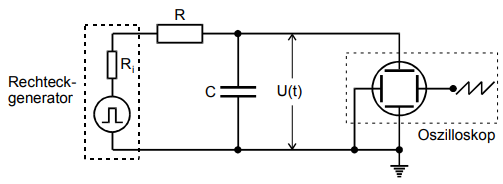
\includegraphics{V353_1.png}
  \caption{Messschaltung zur Bestimmung der Zeitkonstanten mittels Beobachtung des 
  Entladevorgangs. \cite[S. 6]{kent}}
  \label{fig:v353_1}
\end{figure}

%2.2
\subsection{Messreihe zur Bestimmung der Spannungsamplitude des Kondensators
im RC-Kreis}
Für die zweite Messreihe wird eine Sinusspannung $U_\text{0}(t)$ angelegt und die 
Amplitude $A$ der Kondensatorspannung $U_\text{C}(t)$ für dieselben Frequenzen $\omega$ festgehalten.

%2.3
\subsection{Messreihe zur Bestimmung der Phasenverschiebung im RC-Kreis}
In der dritten Messreihe wird die Phasenverschiebung $\phi$ zwischen der generierten 
Spannung $U_\text{G}(t)$ und der Kondensatorspannung $U_\text{C}(t)$ bestimmt.
Hierzu wird die Schaltung so verändert, dass die generierte Spannung ebenfalls auf 
dem Oszilloskopen dargestellt werden kann (Abbildung \ref{fig:v353_3}) und die Signale 
werden übereinander 
symmetrisch zur $t$-Achse ausgelegt. Mithilfe der Cursor-Funktion wird nun der Abstand
$a$ zwischen den zugehörigen Nulldurchläufen gemessen (Abbildung \ref{fig:phi}), wobei
die Periodendauer $b$ durch die Frequenz $\omega$ gegeben ist.
\begin{figure}[H]
  \centering
  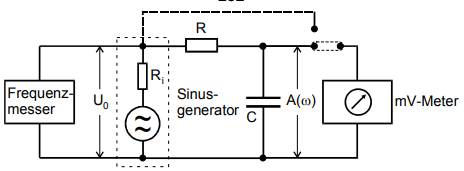
\includegraphics{V353_2.png}
  \caption{Messschaltung zur Bestimmung der Phasenverschiebung $\phi$. \cite[S. 7]{kent}}
  \label{fig:v353_3}
\end{figure}
\begin{figure}
  \centering
  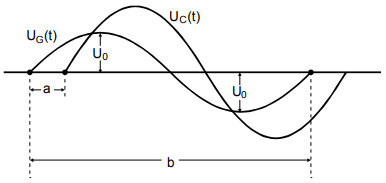
\includegraphics{phi.png}
  \caption{Messung der Phasenverschiebung zwischen zwei Spannungen mit dem
Zweistrahloszilloskopen. \cite[S. 7]{kent}}
  \label{fig:phi}
\end{figure}

%2.4
\subsection{Messreihe zur Bestätigung der Integratorfunktion des RC-Kreises}
Um die Integratorfunktion des RC-Kreises zu überprüfen, wird nun eine ausreichend hohe
Frequenz $\omega$ eingestellt und eine Rechteckspannung angelegt. Das Oszilloskop 
zeigt nun sowohl die angelegte als auch die integrierte Spannung an. Als zweites wird eine
Dreieckspannung angelegt. Die letzte Einstellung ist eine Sinusspannung. Die Ergebnisse
werden als Bilder gespeichert.